\section{绪论}

\subsection{细胞大小的决定}

一般认为,细胞的大小取决于核糖体的活性,因为蛋白质的量由核糖体决定。最小的细胞是支原体。

从果蝇到哺乳动物,都应用一套几乎完全相同的信号网络来调控细胞大小。在哺乳动物中,这一网络的中心是一个名为mTOR(哺乳动物雷帕霉素靶蛋白\footnote{Mammalian target of rapamycin,因其能被雷帕霉素抑制得名。})的蛋白激酶。如果mTOR失活,细胞体积缩小。(\autoref{fig:mtor})

\begin{figure}[htbp]
	\centering
	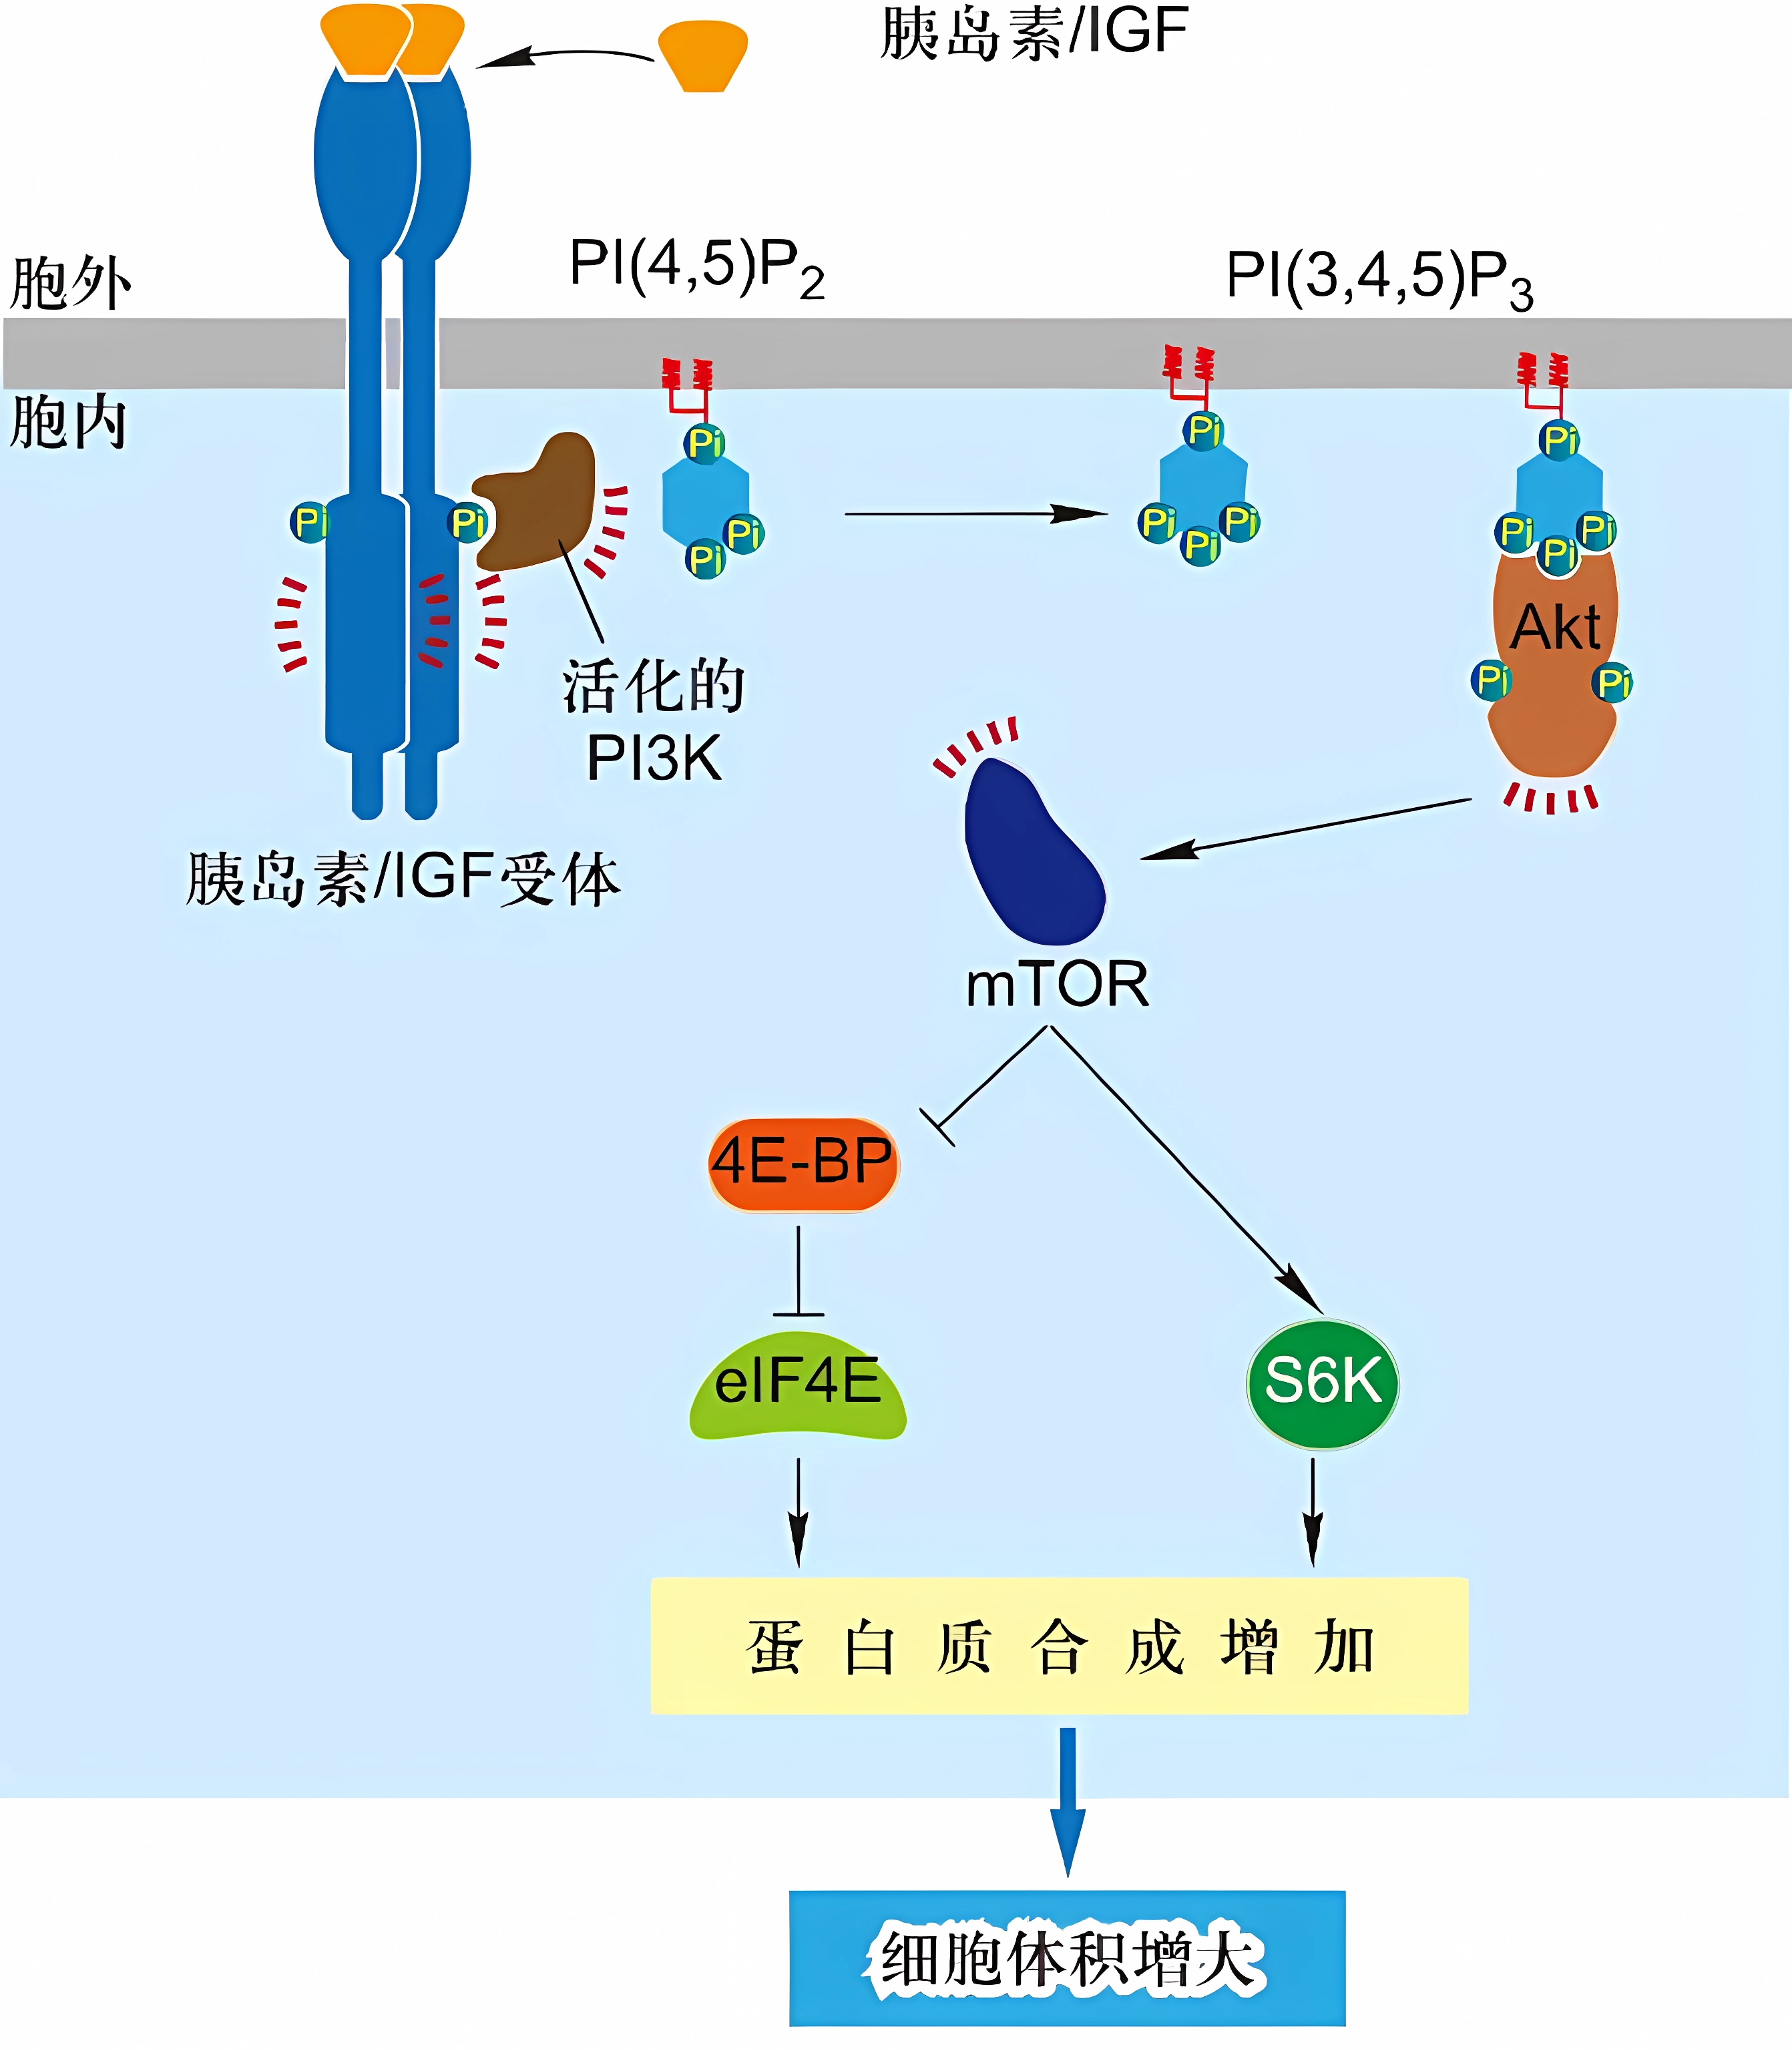
\includegraphics[width=0.5\textwidth]{Pics/mTOR}
	\caption{调控细胞大小的信号网络}
	\label{fig:mtor}
\end{figure}

\begin{figure}[htbp]
	\centering
	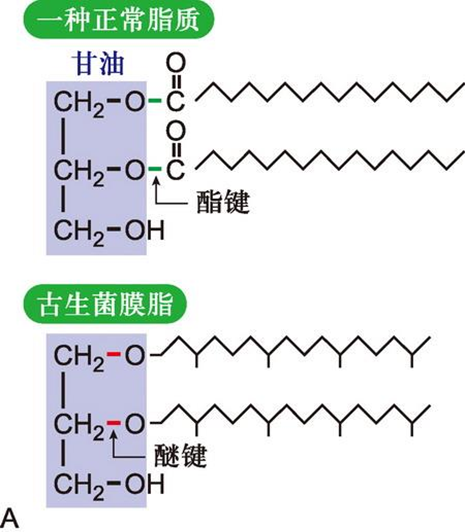
\includegraphics[width=.3\textwidth]{Pics/古细菌的细胞膜}
	\caption{古细菌膜脂的醚键}
	\label{fig:archaealMembraneLipidEtherBonds}
\end{figure}

细胞的大小还与其他因素有关,如植物细胞里液泡体积增大也会使细胞体积增大。

\subsection{古细菌(古核细胞)}

通过直系同源基因相似性比较,发现古细菌和真细菌在很早就分化了。很多古细菌都生活在极端环境中。

古细菌的特点:

\begin{description}
	\item[细胞壁] 古细菌的细胞壁没有胞壁酸或肽聚糖,革兰氏染色呈阴性或阳性。
	\item[细胞质膜] 古细菌的膜脂是以醚键(\autoref{fig:archaealMembraneLipidEtherBonds})与甘油结合,膜脂中还含有鲨烯衍生物,是一种非极性脂质。
	\item[基因结构] 与细菌相似之处是:环状DNA、有操纵子、大部分无内含子、具多顺反子;与真核生物相似之处是:类似核小体的结构、部分基因有内含子、RNA聚合酶为复杂多聚体、翻译起始氨基酸是Met;
	\item[核糖体] 古核生物的核糖体与真核生物更接近,但多数古核生物核糖体是70S。抑制细菌核糖体的药物对古菌无效。
\end{description}

古核生物、原核生物、真核生物的比较见\autoref{tab:三种细胞的比较}。

\begin{table}[htbp]
\centering
\begin{tabularx}{\textwidth}{|C|c|c|c|}
	\hline
	\textbf{特征} & \textbf{原核细胞} & \textbf{古核细胞} & \textbf{真核细胞} \\ \hline
	细胞膜 & \cellcolor{blue!40}多功能 & \cellcolor{blue!40}多功能 & 功能少 \\ \hline
	核膜 & \cellcolor{blue!40}无 & \cellcolor{blue!40}无 & 有 \\ \hline
	核DNA & \cellcolor{blue!40}单个(少数多个)环状 & \cellcolor{blue!40}单个环状 & 多条线性 \\ \hline
	组蛋白 & 无或少有 & \cellcolor{red!40}有 & \cellcolor{red!40}有 \\ \hline
	核仁 & \cellcolor{blue!40}无 & \cellcolor{blue!40}无 & 有 \\ \hline
	核糖体 & \cellcolor{blue!40}70S=50S+30S & \cellcolor{blue!40}70S=50S+30S\footnotemark & 80S=60S+40S \\ \hline
	核糖体对氯霉素 & 敏感 & \cellcolor{red!40}不敏感 & \cellcolor{red!40}不敏感 \\ \hline
	翻译起始 & fMet & \cellcolor{red!40}Met & \cellcolor{red!40}Met \\ \hline
	膜质细胞器 & \cellcolor{blue!40}无 & \cellcolor{blue!40}无 & 有 \\ \hline
	质DNA & \cellcolor{blue!40}质粒 & \cellcolor{blue!40}质粒 & 线粒体,叶绿体 \\ \hline
	细胞壁 & 主要是肽聚糖 & 蛋白质 & 多样 \\ \hline
	细胞骨架 & 有 & 有 & 有 \\ \hline
	增殖方式 & \cellcolor{blue!40}无丝分裂 & \cellcolor{blue!40}无丝分裂 & 有丝分裂为主 \\ \hline
\end{tabularx}
\caption{三种细胞的比较}
\label{tab:三种细胞的比较}
\end{table}
\footnotetext{古菌的核糖体虽然与原核生物沉降系数相同,\zhongdian{但是其蛋白质组成与真核细胞更接近。}}

\section{细胞质膜}

\subsection{细胞质膜的结构}

\subsubsection{结构模型}

用锇酸固定细胞,由于锇酸与磷脂分子头部亲和力强,所以形成电镜中“暗-亮-暗”三层条带。(\autoref{fig:plasma_menb_em})

\begin{figure}[htbp]
	\centering
	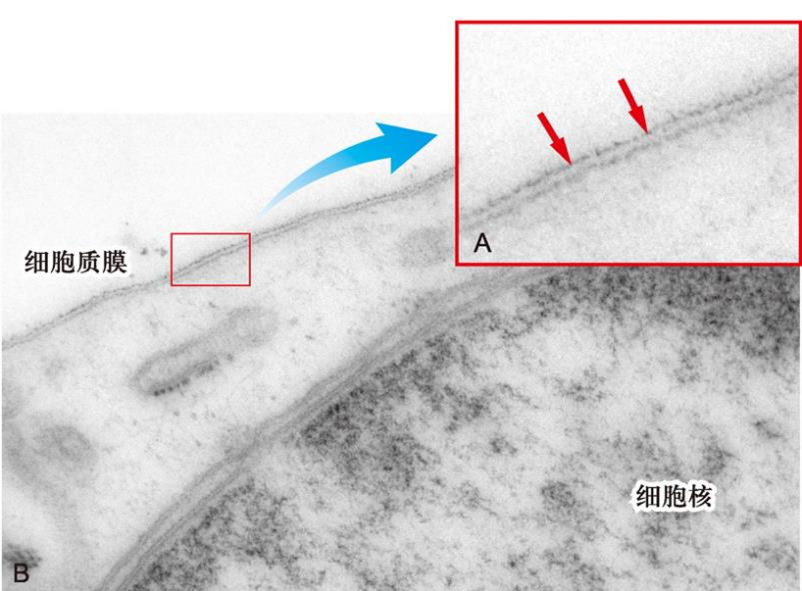
\includegraphics[width=0.5\linewidth]{Pics/电镜下的细胞质膜}
	\caption{电镜下的细胞质膜}
	\label{fig:plasma_menb_em}
\end{figure}

\paragraph{流动镶嵌模型}

在三明治模型、单位膜模型的基础上,Robertson提出了流动镶嵌模型。要点有:
\begin{itemize}
	\item 膜的流动性;
	\item 膜蛋白分布的不对称性。
\end{itemize}

\paragraph{脂筏模型}

脂筏模型是对膜流动性的新理解。脂筏模型认为:在脂双层上漂浮着小船一样的胆固醇、鞘磷脂的富集区域,载着可执行特定功能的膜蛋白。

\paragraph{目前对膜结构的认识}

\begin{itemize}
	\item 磷脂双分子层构成生物膜的基本结构。脂筏中存在有助于维持脂筏稳定的蛋白。
	\item 蛋白质镶嵌或结合在脂双层中或表面,赋予生物膜各自的功能。
	\item 膜中生物大分子的互相作用限制了膜的流动性,也形成了许多特殊结构(如耳蜗微绒毛)。
	\item 膜处在不断变化之中,保证了代谢活动正常进行。
\end{itemize}

\subsubsection{膜脂}

膜脂是生物膜的基本组成成分。

\begin{table}[htbp]
	\centering
	\begin{tabularx}{\textwidth}{|C|c|c|c|c|}
		\hline
		蛋白 & 膜脂 & 化学键 & 位置 & 实例 \\ \hline
		N-Gly & 豆蔻酸 & 酰胺键 & 内侧 & Bid \\ \hline
		Cys-SH、Ser/Thr-OH & 软脂酸 & (硫)酯键 & 内侧 & PSD\footnotemark \\ \hline
		Cys-SH & 异戊二烯脂 & 硫酯键 & 内侧 & Ras \\ \hline
		C端氨基酸 & 磷酸乙醇胺、糖基化PI & 酰胺键 & 外侧 & 精卵融合 \\ \hline
	\end{tabularx}
	\caption{脂锚定膜蛋白的类型}
	\label{tab:脂锚定膜蛋白的类型}
\end{table}
\footnotetext{PSD在突触后膜调节NMDA、AMPA等受体活性,提高受体敏感性。}




\section{物质跨膜运输}

\section{细胞质基质与内膜系统}

\section{蛋白质分选与膜泡运输}

\subsection{蛋白质分选}

\subsubsection{蛋白质分选信号}

蛋白质分选信号是位于肽链N端、C端或中间的序列,指导蛋白质的去处。从空间结构上可以分为两类:

\begin{itemize}
	\item 一类为\zhongdian{连续的氨基酸序列},完成分选过程后,有些会被切除;
	\item 一类为\zhongdian{三维结构的信号斑},是在蛋白折叠完成后,表面原子按一定空间结构排布形成。形成信号斑的氨基酸残基可能在线性氨基酸序列上相距很远。\zhongdian{信号斑不被切除}(就算想切除也做不到)。
\end{itemize}

在连续的氨基酸序列中,有导肽和信号肽两类:

\begin{itemize}
	\item 信号肽是靶向内质网的,参与共翻译转运途径;
	\item 导肽(统称)是靶向线粒体、叶绿体、过氧化物酶体等的,参与翻译后转运途径。
\end{itemize}

靶向各细胞器的序列特征如\autoref{tab:靶向细胞器的蛋白质信号序列特征}所示。

\begin{table}[htbp]
	\centering
	\begin{tabularx}{\textwidth}{|c|c|c|C|}
		\hline
		靶细胞器 & 信号序列位置 & 切除 & 信号序列性质 \\ \hline
		内质网 & N 端 & 是 & 碱性氨基酸+疏水氨基酸 \\ \hline
		线粒体 & N 端 & 是 & 两亲$\upalpha$-螺旋 \\ \hline
		叶绿体 & N 端 & 是 & 没有共同基序 \\ \hline
		过氧化物酶体 & 多在 C 端 & 否 & PTS1(SKL)在C端,PTS2在N端 \\ \hline
		细胞核 & 变化的 & 否 & 含有短的富含Lys和Arg残基序列 \\ \hline
	\end{tabularx}
	\label{tab:靶向细胞器的蛋白质信号序列特征}
	\caption{靶向细胞器的蛋白质信号序列特征}
\end{table}
\subsubsection{蛋白质分选的基本类型}

\subsubsection{蛋白质向线粒体和叶绿体的分选}

\begin{figure}[htbp]
	\centering
	\includegraphics[width=\linewidth]{Pics/核基因编码的线粒体蛋白转运}
	\caption{核基因编码的线粒体蛋白转运}
	\label{fig:tim_tom}
\end{figure}

\subsection{细胞内膜泡运输}

细胞内膜泡运输需要多种转运膜泡参与,根据表面包被蛋白的不同,分为COP II包被膜泡、COP I包被膜泡、网格蛋白/接头蛋白(clathrin/AP)包被膜泡三类。




\section{线粒体和叶绿体}

\subsection{线粒体}

\subsubsection{线粒体的融合与分裂}

线粒体频繁的融合与分裂被认为是线粒体形态调控的基本方式,数目调控的基础。

频繁的线粒体融合与分裂实际上把线粒体联系成一个动态整体。植物细胞中,可见线粒体融合与分裂的偶联现象,生物学意义可能是共享遗传信息,植物中多个线粒体才共享一个DNA分子。

介导线粒体融合和分裂的两类蛋白质均是大分子GTP酶。

\paragraph{线粒体融合}

介导线粒体融合的蛋白质定位于线粒体外膜,在果蝇中是Fzo,在哺乳动物中是Mfn。虽然名字不同,但线粒体融合的分子机制高度保守。

虽然植物细胞中存在频繁的线粒体融合与分裂现象,但是基因组中并不存在\textit{Fzo}或\textit{Mfn}的同源基因。

目前没有发现线粒体融合的结构装置。

\paragraph{线粒体分裂}

在植物和动物细胞中,线粒体的分裂离不开发动蛋白。发动蛋白还介导许多膜相细胞器的融合与断裂,在膜泡运输中也发挥重要作用。

发动蛋白不像Mfn那样具有膜定位能力,需要借助Fis1和Mdv1来招募。

线粒体分裂装置则比较突出,称为线粒体分裂环,分为外环和内环。外环在线粒体外膜表面,内环在线粒体内膜之下。

\subsubsection{线粒体的超微结构}

线粒体的结构包含外膜、膜间隙、内膜和基质。外膜平展,内膜凹陷成嵴,\zhongdian{动物细胞常见规则折叠而成的“袋状嵴”,植物细胞常见不规则折叠而成的“管状嵴”}。

\begin{description}
	\item[外膜] 外膜上分布着\zhongdian{孔蛋白构成的通道,可开闭}。外膜通透性很高,离子环境几乎与细胞质基质相同。外膜的标志酶是单胺氧化酶。
	\item[膜间隙] 呼吸加强时,膜间隙可扩大。标志酶是腺苷酸激酶,催化ATP+AMP$\longrightarrow$2ADP。
	\item[内膜]
\end{description}

\section{细胞骨架}

细胞骨架,由粗到细包括:微管(MT)、中间丝(IF)、微丝(MF)。(\autoref{fig:cytoskeleton})细胞骨架与数目众多的结合蛋白的相互作用,是细胞结构与功能相统一的分子基础。

\begin{figure}[h]
	\centering
	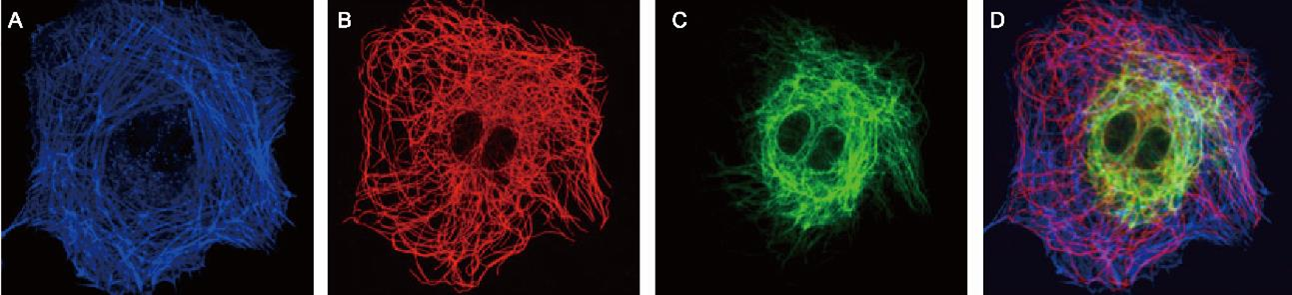
\includegraphics[width=0.9\linewidth]{Pics/cytoskeleton}
	\caption{免疫荧光染色示微丝(A)、微管(B)、中间丝(C)在体外培养的小鼠上皮细胞内的分布,以及叠加图(D)}
	\label{fig:cytoskeleton}
\end{figure}


\subsection{微丝}

微丝又称肌动蛋白丝,存在于所有真核细胞内。

它的空间结构与功能取决于与之结合的微丝结合蛋白。在三类细胞骨架中,微丝更接近细胞的边缘。(\autoref{fig:cytoskeleton})

以下活动有微丝的参与:细胞突起(微绒毛、伪足)、胞质分裂、吞噬作用、细胞迁移、肌球蛋白运动(如肌细胞收缩)、细胞收缩、依赖肌球蛋白的物质运输等。

\begin{figure}[htbp]
	\centering
	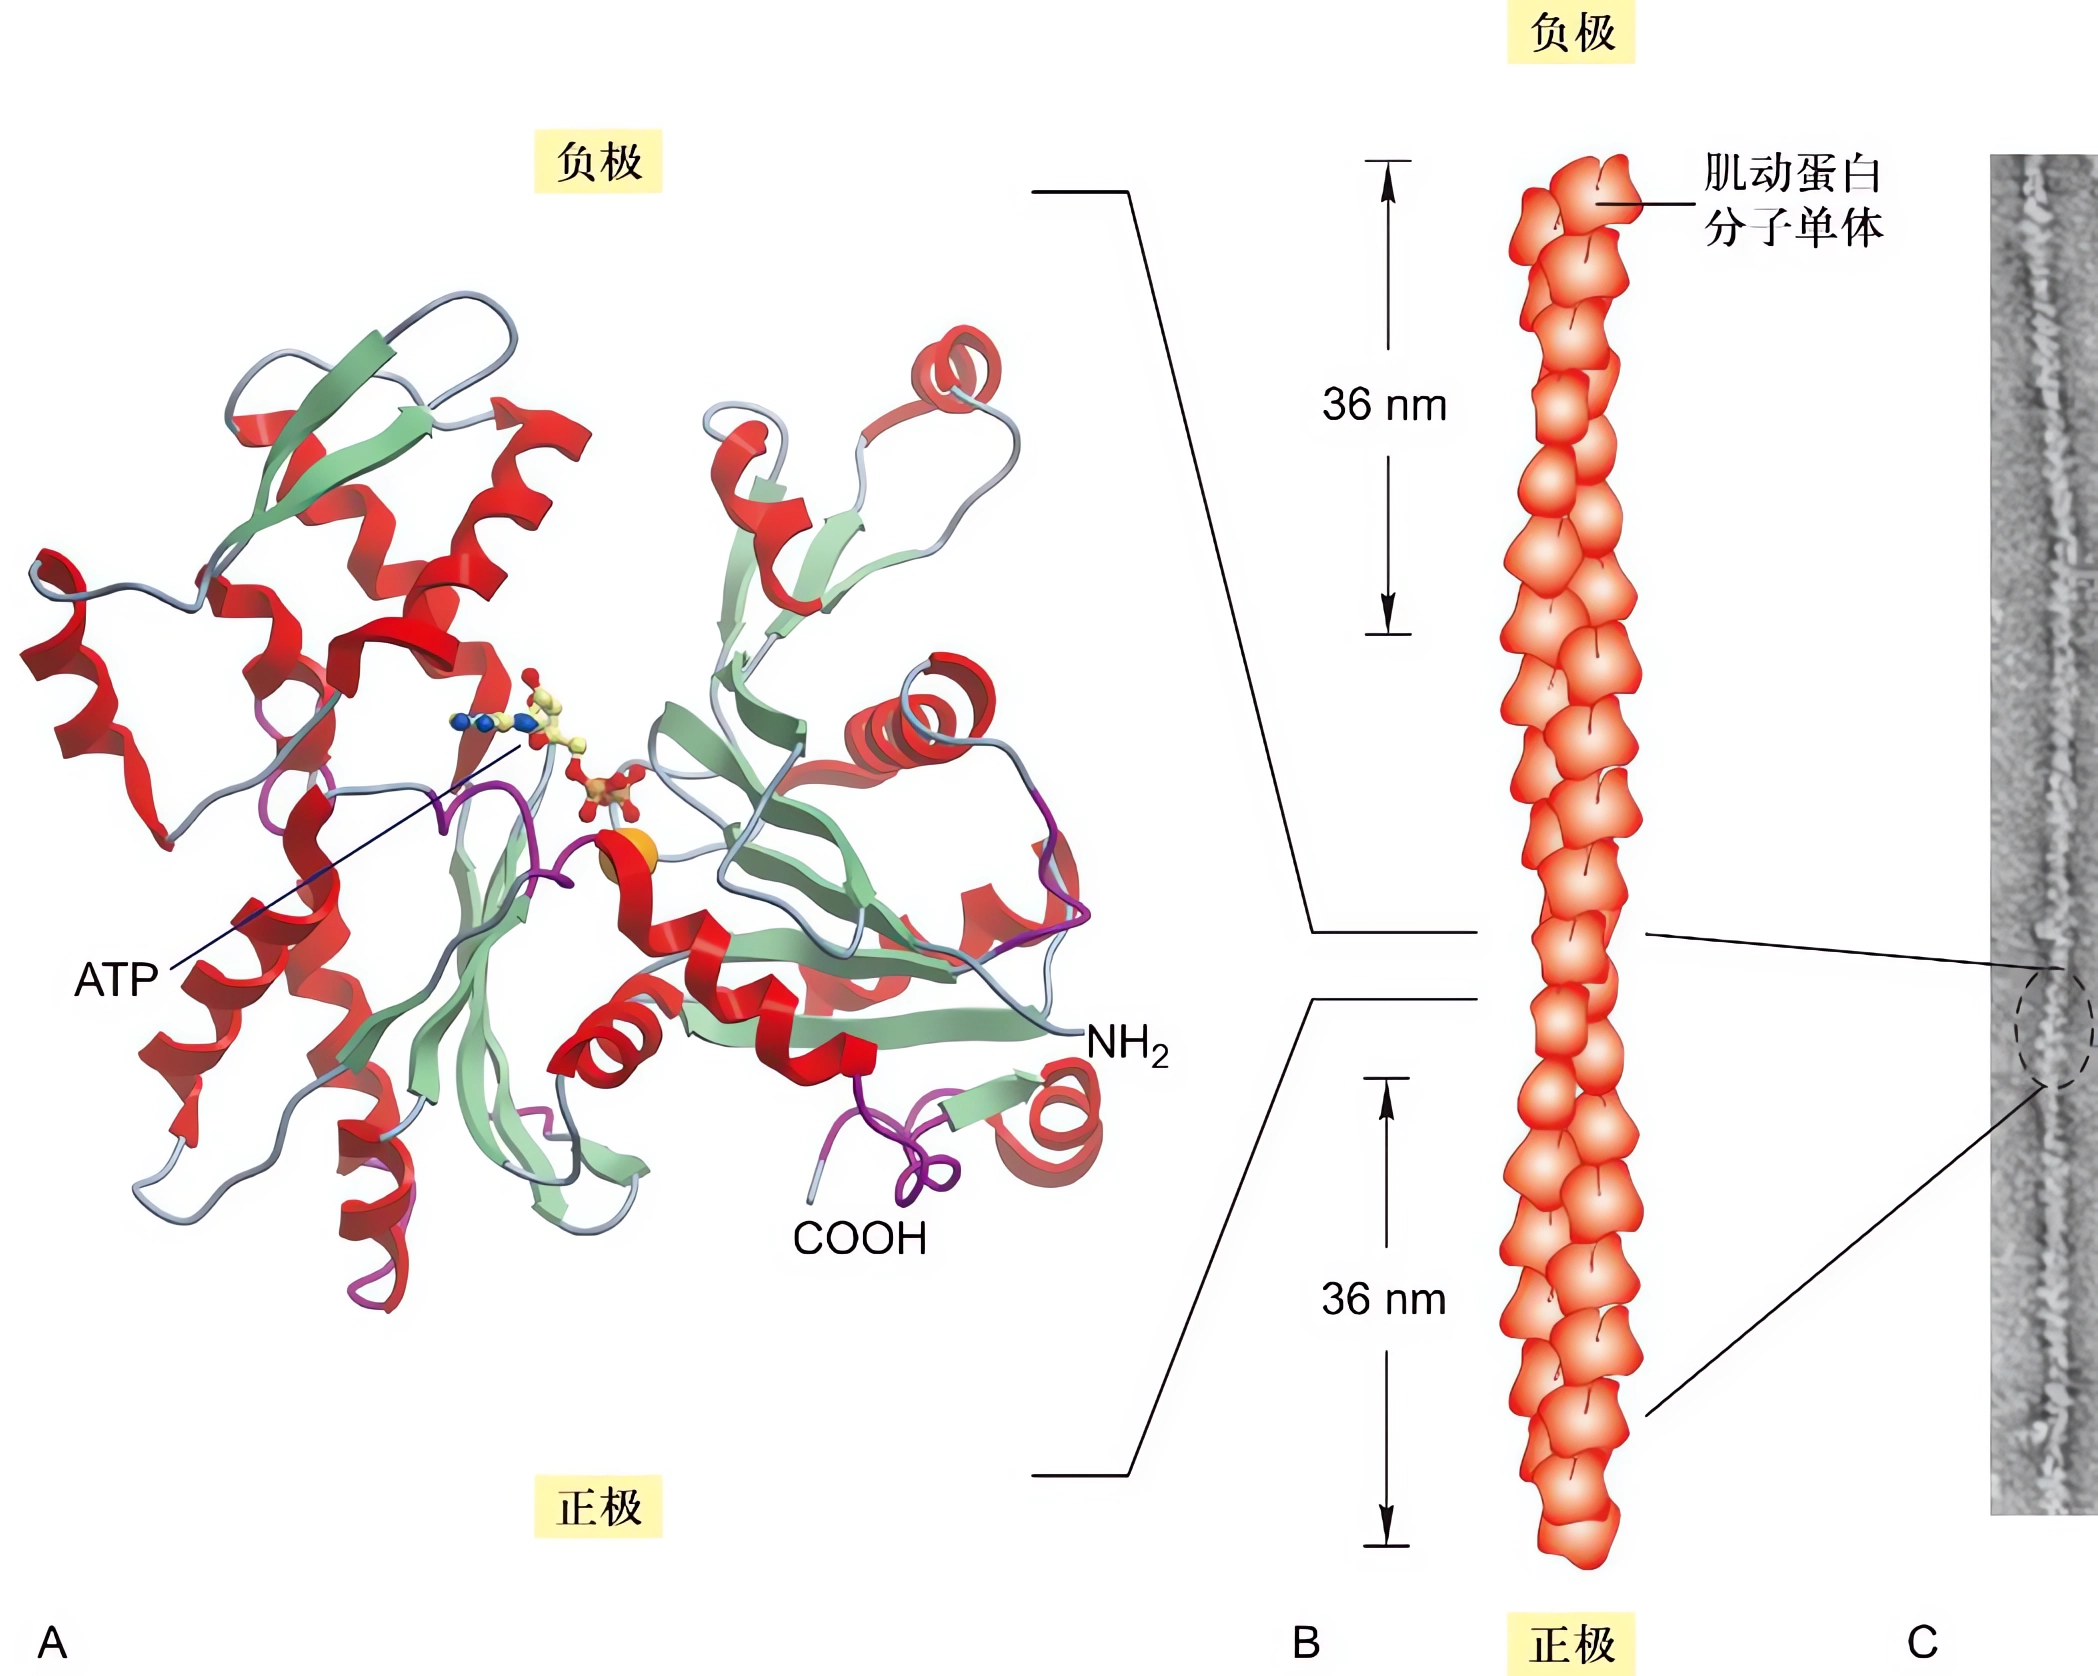
\includegraphics[width=0.7\linewidth]{肌动蛋白和微丝}
	\caption{肌动蛋白单体和微丝}
	\label{fig:actin_microfibre}
\end{figure}

\subsubsection{微丝的组成}

微丝是两股F-actin组成的右手螺旋,具有极性,肌动蛋白单体有裂缝的一端称为负极,另一端为正极。主要成分是肌动蛋白(actin),肌动蛋白是细胞内含量最多的蛋白质之一\footnote{常用作WB的内参。}。

肌动蛋白在细胞内以球状肌动蛋白(G-actin)的单体和纤维状肌动蛋白(F-actin)的多聚体形式存在。

肌动蛋白单体的裂缝可以容纳\underline{ATP}/ADP和\ce{Ca^{2+}}/\underline{\ce{Mg^{2+}}}。肌动蛋白常是与画下划线的那个结合。

按照等电点分为$\upalpha$、$\upbeta$、$\upgamma$三种,等电点高低:$\upalpha>\upgamma>\upbeta$。

\begin{itemize}
	\item $\upalpha$-actin主要分布在肌细胞中,如心肌细胞、肠道平滑肌;
	\item $\upbeta$-actin主要分布在细胞的边缘;
	\item $\upgamma$-actin是应力纤维的组成成分。
\end{itemize}

原核生物也存在肌动蛋白的类似物,如MreB。



\subsubsection{微丝的组装过程}

通常只有结合ATP的肌动蛋白单体才参与微丝组装。微丝的组装受到胞内环境的影响:

\begin{itemize}
	\item \ce{Ca^{2+}}多,\ce{Na+}、\ce{K+}少,倾向于解聚;
	\item \ce{Mg^{2+}}、ATP、\ce{Na+}、\ce{K+}多,倾向于聚合。
\end{itemize}

肌动蛋白的组装分为下列几个步骤:

\begin{description}
	\item[成核反应] 如同DNA不能从头合成而需要引物,肌动蛋白单体不能直接从头组装。游离的G-actin与Arp2/3复合物(肌动蛋白相关蛋白)共同参与成核。
\end{description}
\section{细胞核、染色质}

\section{核糖体}

\section{细胞信号转导}

\section{细胞周期、细胞分裂}

\section{细胞增殖调控与癌细胞}





\section{细胞分化、干细胞}

\section{细胞衰老与细胞程序性死亡}

\subsection{细胞程序性死亡}

\begin{itemize}
	\item 炎症caspase:1、4、5、11、12;
	\item 凋亡起始caspase:2、8、9、10;
	\item 执行caspase:3、6、7。
\end{itemize}


\section{细胞的社会联系}

\subsection{细胞连接}

细胞连接是细胞之间、细胞与胞外基质相连接的结构。细胞连接包括下面三类:

\begin{description}
	\item[封闭连接] 将相邻上皮细胞的质膜紧紧地连接在一起,阻止小分子物质通过。如紧密连接。
	\item[锚定连接] 将细胞与相邻细胞或胞外基质连接。组分有胞内骨架、跨膜蛋白、胞外结构。
	\item[通信连接] 介导相邻细胞的物质转运或化学、电信号的传递。如间隙连接、化学突触、电突触(间隙连接)。
\end{description}

\subsubsection{封闭连接——以紧密连接为例}

关键结构是相邻细胞膜上跨膜蛋白形成的嵴线,

\subsubsection{锚定连接}

\begin{table}[htbp]
	\centering
	\begin{tabularx}{\textwidth}{|c|C|C|c|}
		\hline
		连接类型 & 骨架结构 & 跨膜蛋白 & 胞外结构 \\ \hline
		桥粒 & 中间丝 & 钙黏蛋白 & 相邻细胞 \\ \hline
		半桥粒 & 中间丝 & 整联蛋白 & 层粘连蛋白 \\ \hline
		黏着带 & 微丝 & 钙黏蛋白 & 相邻细胞 \\ \hline
		黏着斑 & 微丝 & 整联蛋白 & 胶原、纤连蛋白 \\ \hline
	\end{tabularx}
	\caption{锚定连接的类型}
	\label{tab:锚定连接的类型}
\end{table}

\subsection{细胞黏着}

\begin{table}[htbp]
	\centering
	\begin{tabularx}{\textwidth}{|c|C|C|C|c|}
		\hline
		CAM家族 & 配对 & 离子依赖 & 胞内骨架 & 细胞连接 \\ \hline
		钙黏蛋白 & 同亲 & + & 微丝、中间丝 & 黏着带、桥粒 \\ \hline
		选择素 & 异亲 & + & 微丝 & --- \\ \hline
		IgSF & 同亲 & - & --- & --- \\ \hline
		整联蛋白 & 异亲 & + & 微丝、中间丝 & 黏着斑、半桥粒 \\ \hline
	\end{tabularx}
	\caption{细胞黏着蛋白的分类}
	\label{tab:细胞黏着蛋白的分类}
\end{table}

\begin{table}[htbp]
	\centering
	\begin{tabularx}{\textwidth}{|c|C|c|}
		\hline
		名称 & 主要分布 & 参与细胞连接类型 \\ \hline
		E-钙黏蛋白 & 上皮细胞 & 黏着连接 \\ \hline
		N-钙黏蛋白 & 神经、心脏、骨骼肌及成纤维细胞 & 黏着连接、化学突触 \\ \hline
		P-钙黏蛋白 & 胎盘、表皮 & 黏着连接 \\ \hline
		VE-钙黏蛋白 & 内皮细胞 & 黏着连接 \\ \hline
	\end{tabularx}
	\caption{钙黏蛋白的分类}
	\label{tab:钙黏蛋白的分类}
\end{table}